
% ------------------------------------------------------------------------------
\section{Obsidian: a domain specific embedded language for GPU programming}
\label{sec:obsidian}

To introduce Obsidian, we consider the implementation of a parallel prefix 
kernel. The implementation bears a close resemblance to the Lava implementation 
from section~\ref{sec:combinators}:

                                   
% ------------------------------------------------------------------------------
%sklansky :: (Choice a, Syncable (Arr s a)) => 
%            Int -> (a -> a -> a) -> Arr s a -> W (Arr s a) 
%sklansky 0 op = return 
%sklansky n op = two (sklansky (n-1) op) ->- sfan ->- sync
%    where sfan arr = do 
%            (a1,a2) <- halve arr
%            let m = len a1
%                c = a1 ! (m-1)
%            a2' <- fun (op c) a2
%            conc (a1,a2')


\begin{code}
sklansky :: (Choice a, Syncable (Arr s a)) => 
             (a -> a -> a) -> Arr s a -> W (Arr s a) 
sklansky op arr 
   | len arr == 1 = return arr
   | otherwise = (two (sklansky op) ->- sfan ->- sync) arr
    where sfan arr = do 
            (a1,a2) <- halve arr
            let m = len a1
                c = a1 ! (fromInt (m-1))
            a2' <- fun (op c) a2
            conc (a1,a2')

\end{code}
% ------------------------------------------------------------------------------
The most notable differences between the two implementations are that Obsidian 
functions are monadic and that a datatype {\tt Arr} is used where Haskell lists
are used in Lava. The pattern matching on the list used in Lava is here 
replaced by guards. The function {\tt len :: Arr s a -> Int} gives the 
length of the array. These differences lead to a slightly different programming
style.

%Another effect
%of using the {\tt Arr} type rather than lists is the need to pass a size
%parameter to the {\tt sklansky} function.  However, this limitation comes from 
%a design decision that may be subject to change shortly. 

The Obsidian version of the {\tt sklansky} function implements the sought
recursive parallel prefix algorithm, but it 
contains no information about where in the memory hierarchy the intermediate
results are to be held. The following program uses {\tt sklansky} from 
above but turns it into a concrete kernel that computes all the partial sums
of an array of integers: 

% ------------------------------------------------------------------------------
\begin{code}
scan_add_kernel :: GArr IntE -> W (GArr IntE) 
scan_add_kernel = cache ->- sklansky (+) ->- wb ->- sync
\end{code}
% ------------------------------------------------------------------------------
The function {\tt cache} specifies that if the array is stored it should be
stored in the on-chip shared memory. Actually storing an array is done using
the {\tt sync} function, which functionally is the identity function, but has
the extra effect of synchronising all processes after writing their data in
shared memory, such that they can exchange intermediate results. Using {\tt
sync} here allows for computations or transformations to be performed on the
data as it is being read in from global device memory. In the {\tt
scan\_add\_kernel} above this means that the first {\tt sklansky} stage will
be computed with global data as input, putting its result into shared memory.
A kernel computing the same thing but using the memory differently can be
implemented like this:
% ------------------------------------------------------------------------------
\begin{code}
scan_add_kernel2 :: GArr IntE -> W (GArr IntE) 
scan_add_kernel2 = cache ->- sync ->- sklansky (+) ->- wb ->- 
                     sync
\end{code}
% ------------------------------------------------------------------------------
Here the array is first stored into shared memory. The {\tt sklansky} stages
are then computed entirely in shared memory. The write-back function, {\tt wb}, 
works in a very similar way but specifies that the array should be moved back 
into the global memory. 

Now, {\tt scan\_add\_kernel} can be launched on the GPU from within a GHCI 
session using a function called {\tt execute}:

% ------------------------------------------------------------------------------
\begin{code}
execute :: ExecMode -> (GArr (Exp a) -> W (GArr (Exp b)) -> 
              [Exp a] -> IO [Exp b]
\end{code}
% ------------------------------------------------------------------------------
Here {\tt ExecMode} can be either {\tt GPU} for launching the kernel on the 
GPU or {\tt EMU} for running it in emulation mode on the system's CPU. Below is 
the result\footnote{The output has been shortened to fit on a line.} of 
launching the scan kernel on example input:

% ------------------------------------------------------------------------------

%  \DefineVerbatimEnvironment
%     {code}{Verbatim}
%     {fontsize=\small,xleftmargin=0.6cm,samepage=true}

%\begin{small}


\begin{code}
*Main> execute GPU scan_add_kernel [1..256]
[0,1,3,6,10,15, ... ,32131,32385,32640] 
\end{code}

%\end{small}
% [E (LitInt 1),E (LitInt 3),E (LitInt 6), ... ,E (LitInt 32896)] 
% ------------------------------------------------------------------------------

Beyond the combinators described so far, we have experimented with combinators 
and permutations  needed for certain iterative sorting networks. Amongst these 
are {\tt evens} that applies a function to each pair of elements of an array. 
Together with {\tt rep} that repeats a computation a given number of times and 
a permutation called {\tt riffle} a shuffle exchange network can be defined: 

% ------------------------------------------------------------------------------

\begin{code}
shex n f = rep n (riffle ->- evens f ->- sync)
\end{code}

% ------------------------------------------------------------------------------
The shuffle exchange network can be used to implement a merger useful in sorters. 


% ------------------------------------------------------------------------------
\subsection{Implementation} 

As seen in the examples, an Obsidian program is built from functions between 
arrays. These arrays are of type {\tt Arr s a}. There are also type synonyms
{\tt GArr} and {\tt SArr} implemented as follows: 

% ------------------------------------------------------------------------------
\begin{code}
data Arr s a = Arr (IxExp ->  a, Int)
type GArr a = Arr Global a
type SArr a = Arr Shared a 
\end{code}
% ------------------------------------------------------------------------------
In Obsidian an array is represented by a function from indices to values and an 
integer giving the length of the array.

In most cases the {\tt a} in {\tt Arr s a} will be of an expression type: 
\begin{code} 
data DExp = LitInt Int
          | LitBool Bool
          | LitFloat Float 
          | BinOp Op2 DExp DExp 
          | UnOp  Op1 DExp 
          | If DExp DExp DExp 
          | Variable Name 
          | Index DExp DExp  
            deriving(Eq,Show)
\end{code} 

The above expressions are dynamic in the sense that they can be used to 
represent values of {\tt Int}, {\tt Float} and {\tt Bool} type. 
This follows the approach from Compiling Embedded Languages 
\cite{Elliott03:CompileDSEL-JFP}. However, 
to obtain a typed environment in which to operate, phantom types are used. 

\begin{code} 
type Exp a = E DExp

type IntE   = Exp Int
type FloatE = Exp Float
type BoolE  = Exp Bool
type IxExp  = IntE 
\end{code}

As an example consider the program: 
% ------------------------------------------------------------------------------
\begin{code} 
add_one :: GArr IntE -> W (GArr IntE)
add_one = fun (+1) ->- sync
\end{code} 
% ------------------------------------------------------------------------------
This program adds 1 to each element of an array of integers. The function {\tt fun}
has type {\tt (a -> b) -> Arr s a -> Arr s b}. {\tt fun} performs for arrays what 
{\tt map} does for lists. 
The {\tt sync} function used in the example has the effect that
the array being synced upon is written to memory. At this point the type of 
the array determines where in memory it is stored. An array of type {\tt SArr} 
will end up in the {\em shared memory} (which is currently 16KB per multi-processor). 
In this version of Obsidian it is up to the programmer to make sure that the 
array fits in the memory. An array of type  {\tt GArr} ends up in the global 
device memory, roughly a gigabyte on current graphics cards.  Using {\tt sync} 
can have performance implications since it facilitates sharing of computed 
values. 
%However, functionally it is the identity function.

To generate CUDA code from the Obsidian program {\tt add\_one}, it is applied to
a symbolic array of a given concrete length (in this example 256 elements): 

% ------------------------------------------------------------------------------
\begin{code}
input :: GArr IntE 
input = mkArray (\ix -> (index (variable "input") ix)) 256
\end{code}
% ------------------------------------------------------------------------------

Applying {\tt fun (+1)} to this input array results in an array with the 
following indexing function:
\begin {code}
(\ix -> (E (BinOp Add (Index (Variable "input") ix) (LitInt 1)))) 
\end{code} 

At the code generation phase this function is evaluated using a variable 
representing a thread Id. The result is an expression looking as follows:
\begin {code}
E (BinOp Add (Index (Variable "input") (Variable "tid")) (LitInt 1))
\end{code} 

This expression is a direct description of what is to be computed. 
%Figure~\ref{fig:expressions} illustrates this pictorially.
% ------------------------------------------------------------------------------
%\begin{figure}%
%\begin{center}
%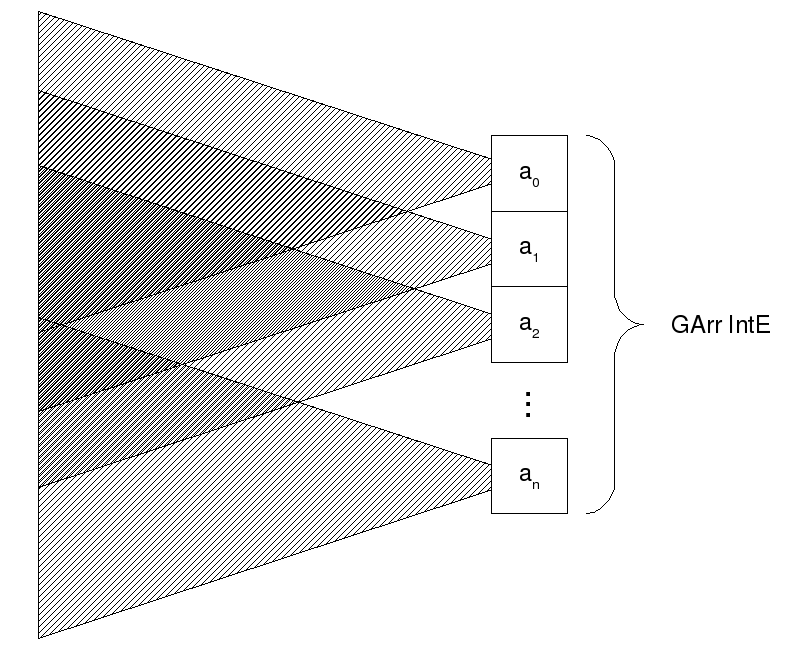
\includegraphics[scale=.25]{expressions.png}
%\caption{Expressions and arrays.}
%\label{fig:expressions}
%\end{center}
%\end{figure} 
% ------------------------------------------------------------------------------



% ------------------------------------------------------------------------------
Importantly, the basic library functions can be implemented using the 
{\tt Arr s a} type and thus be applicable both to shared and global arrays.
The library function {\tt rev} that reverses an array is shown as an example
of this: 

% ------------------------------------------------------------------------------
\begin{code}
rev :: Arr s a -> W (Arr s a) 
rev arr = let n = len arr 
          in  return $ mkArray (\ix -> arr ! ((n - 1) - ix)) n
\end{code}
%$% 
% ------------------------------------------------------------------------------
The function {\tt rev} uses {\tt mkArray} to create an array whose indexing 
function reverses the order of the elements of the given array {\tt arr}. 
The Obsidian program {\tt rev $-$>$-$ sync} 
corresponds\footnote{in the real IC {\tt arrx} and {\tt arry} are replaced by identifiers generated in the{\tt W} monad}
to the following lines of C code:
 
\begin{code}
arrx[ThreadIdx.x] = arry[n - 1 - ThreadIdx.x];  
__syncthreads();
\end{code} 

When an Obsidian function, such as the {\tt scan\_add\_kernel} from the 
previous section, is run, two data structures are accumulated into a monad 
called {\tt W}. The first is intermediate code {\tt IC} and the second a symbol 
table. The {\tt W} monad is a writer monad extended with some extra 
functionality for generating identifier names and to maintain the symbol table. 
You can think of the {\tt W} monad as: 

\begin{code}
type W a = WriterT (IxExp -> IC) (State (SymbolTable,Int)) a
\end{code}

The IC used here is just a list of statements, (less important statements have 
been removed to save space ({\tt ...})). The {\tt IC} contains a 
subset of CUDA. In this version of Obsidian not much more than the 
{\tt Synchronize} and assignment statements of CUDA are used. 
%Looping constructs are not 
%part of the {\tt Statement} type. We are experimenting with 
%generating unrolled loops only: 

% ------------------------------------------------------------------------------
%\begin{samepage}
\begin{code} 
data Statement = Synchronize 
               | DExp ::= DExp 
               -- used later in code generation
               | IfThenElse BoolE [Statement] [Statement]
                 deriving (Show,Eq)

type IC = [Statement]
\end{code} 
%\end{samepage}
% ------------------------------------------------------------------------------

The symbol table is a mapping from names to types and sizes: 
\begin{code} 
type SymbolTable = Map Name (Type,Int) 
\end{code}

Information needs to be stored into the SymbolTable whenever new intermediate
arrays are created. We have chosen to put this power in the hands of the programmer
using the {\tt sync} function. The {\tt sync} function is overloaded for 
a number of different array types: 

%So, how does all the needed information end up in the IC and SymbolTable? 
%This is the responsibility of the {\tt sync} function. The {\tt sync} 
%function is overloaded for a number of different array types: 

\begin{code}
class Syncable a where 
    sync :: a -> W a
    commit :: a -> W a 
\end{code} 

The types of the {\tt sync} and the related {\tt commit} function
are shown in the class declaration above. To illustrate what {\tt sync} does, 
one instance of its implementation is shown: 

\begin{code}
instance TypeOf (Exp a) => Syncable (GArr (Exp a)) where
    sync arr = do
      arr' <- commit arr
      write $ \ix -> [Synchronize]
      return arr'
    commit arr = do 
      let n = len arr
      var  <- newGlobalArray (typeOf (arr ! (E (LitInt 0))))  n 
      write $ \ix -> [(unE (index var ix)) ::= unE (arr ! ix)] 
      return $ mkArray (\ix -> index var ix) n
\end{code}
%$ 

The {\tt sync} function commits its argument array and 
thereafter writes \newline {\tt [Synchronize]} into the W monad. To see what 
this means, one should also look at the {\tt commit} function, in which
a new array is created of the same size and type 
as the given array. In the next step, an assignment statement is written into 
{\tt W} monad (added to the intermediate code). It
assigns the values computed in the given array to the newly created array.
From the intermediate code and the symbol table accumulated into the {\tt W} 
monad, C code is generated following a procedure outlined in 
figure~\ref{fig:code_gen}.
% ------------------------------------------------------------------------------
%\FloatBarrier
\begin{figure}%
\begin{center}
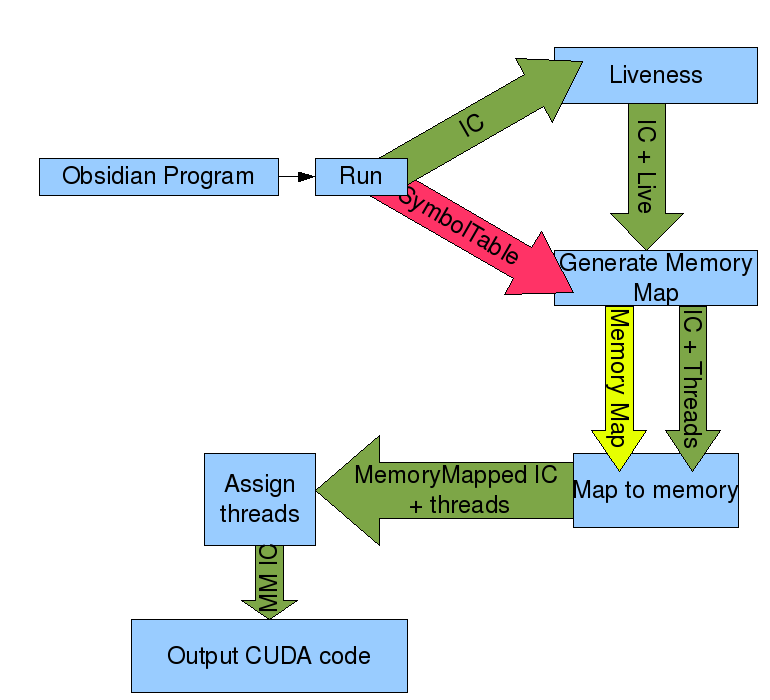
\includegraphics[scale=.3]{./ifl/stages2.png}
\caption{Steps involved in generating CUDA C code from Obsidian description.
The boxes represent functions and the arrows represent data structures.}
\label{fig:code_gen}
\end{center}
\end{figure}
%\FloatBarrier
% ------------------------------------------------------------------------------

The first step depicted in the figure is the running the Obsidian program. 
This builds two data structures {\tt IC} and {\tt SymbolTable}. 
The IC goes through a simple liveness analysis where for each statement
information about what data elements, in this case arrays,  are alive at 
that point is added. An array is alive if it is used in any of the following 
statements or if it is considered a result of the program. The result of this 
pass is a new {\em IC} where each statement also has a set of names pointing 
out arrays that are alive at that point. 


\begin{code} 
type ICLive = [(Statement, Set Name)]
\end{code}

Now, the symbol table together with the {\tt ICLive} object is used to lay out 
the arrays in memory. Arrays that had type {\tt SArr} are assigned storage in 
the shared memory and arrays of type {\tt GArr} in Global memory. The result 
of this stage is a {\em Memory Map}. This is a mapping from names to positions 
in memory. The picture also shows that another output from this stage is 
intermediate code annotated with thread information, call it {\tt ICT}. This 
is now done in a separate pass over the IC but it could be fused with the 
memory mapping stage, saving a pass over the IC. 
The ICT is just a list of statements and the number of threads assigned to 
compute them:

\begin{code}
type ICT = [(Statement,Int)]
\end{code}
% \noindent
This enables the final pass over the IC to move thread information
into the actual IC as conditionals. The resulting IC is used to output
CUDA code. 

To illustrate this, the code generated from a simple Obsidian program is 
shown. The example is very artificial and uses sync excessively in order
to create more intermediate arrays : 

\begin{code}
rev_add :: GArr IntE -> W (GArr IntE)
rev_add = rev ->- sync ->- fun (+1) ->- sync
\end{code}

Figure~\ref{fig:code1} shows the CUDA C code generated from the {\tt rev\_add} 
program. Here it is visible how intermediate arrays are assigned memory in 
global memory. The global memory is pointed to by {\tt gbase}:   

\begin{figure}
\begin{code} 
__global__ static void rev_add(int *source0,char *gbase){
extern __shared__ char sbase[] __attribute__ ((aligned(4)));
const int tid = threadIdx.x;
const int n0 __attribute__ ((unused)) = 256;
((int *)(gbase+0))[tid] = source0[((256 - 1) - tid)];
__syncthreads();
 ((int *)(gbase+1024))[tid] = (((int *)(gbase+0))[tid] + 1);
__syncthreads();
\end{code}
\caption{Generated CUDA code.} 
\label{fig:code1}
\end{figure}

The code in figure~\ref{fig:code1} does however not show how the {\tt ICT} 
is used in assigning work to threads. To show this  a small part of the 
generated CUDA code from the {\tt scan\_add\_kernel} is given in 
figure~\ref{fig:code2}. Notice the conditional {\tt if (tid < 128)}. 
This line effectively shuts down half of the threads. It can also be seen 
here how shared memory is used, pointed to by {\tt sbase}. Moreover, from the 
line with {\tt (63 < 64) ? ...} it becomes clear that there is room for some
obvious optimisations. 

 

\begin{figure}
\begin{code} 
 __syncthreads();
 if (tid < 128){
   ((int *)(sbase+1520))[tid] = ((tid < 64) ?
   ((tid < 64) ?
   ((int *)(sbase+496))[tid] : 
   ((int *)(sbase+752))[(tid - 64)]) : 
   (((63 < 64) ?
   ((int *)(sbase+496))[63] : 
   ((int *)(sbase+752))[(63 - 64)]) + ((tid < 64) ?
   ((int *)(sbase+496))[tid] : 
   ((int *)(sbase+752))[(tid - 64)])));
 }
\end{code} 
\caption{A small part of the CUDA code generated from the recursive implementation of the Sklansky parallel prefix algorithm.}
\label{fig:code2}
\end{figure}
\noindent

 


% ------------------------------------------------------------------------------
\FloatBarrier
